\documentclass[10pt,a4paper]{article}
\usepackage[utf8]{inputenc}
\usepackage[french]{babel}
\usepackage[T1]{fontenc}
\usepackage{amsmath}
\usepackage{amsfonts}
\usepackage{amssymb}
\usepackage{graphicx}

\usepackage{libertine}
\setlength{\parindent}{0cm}
\setlength{\parskip}{1ex plus 0.5ex minus 0.2ex}
\newcommand{\hsp}{\hspace{20pt}}
\newcommand{\HRule}{\rule{\linewidth}{0.5mm}}

\begin{document}

\begin{titlepage}
  \begin{sffamily}
  \begin{center}

    % Upper part of the page. The '~' is needed because \\
    % only works if a paragraph has started.
    
\includegraphics[scale=0.15]{images/tree.jpg}~\\[1.5cm]

    \textsc{\LARGE U-MONS}\\[2cm]

    \textsc{\Large Rapport de project de Structures de données 2}\\[1.5cm]

    % Title
    \HRule \\[0.4cm]
    { \huge \bfseries Priority Search Tree and Windowing\\[0.4cm] }

    \HRule \\[2cm]
    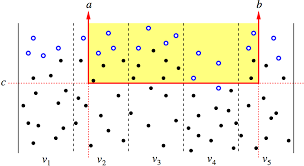
\includegraphics[scale=0.50]{images/window.png}
    \\[2cm]

    % Author and supervisor
    \begin{minipage}{0.4\textwidth}
      \begin{flushleft} \large
        \emph{\textbf{Directeurs :}}\\ G.Devillez et V.Bruyère\\
      \end{flushleft}
    \end{minipage}
    \begin{minipage}{0.4\textwidth}
      \begin{flushright} \large
        \emph{\textbf{Groupe :}}\\ M.Salemi et A.Lecocq
      \end{flushright}
    \end{minipage}

    \vfill

    % Bottom of the page
    {\large \today}

  \end{center}
  \end{sffamily}
\end{titlepage}

\newpage
\tableofcontents
\newpage
\section{Introduction}
    

\subsection{Lecture de l'article}
Durant la phase préliminaire de ce projet, il nous a été demandé de lire une partie d'un article nous donnant toutes les informations et connaissances nécessaires afin de pouvoir commencer notre projet. Nous allons donc ci-dessous rappeler certains des concepts nécessaire à la mise ne pratique de ce travail et la compréhension de celui-ci.
\subsection{Priority Search Tree}
Un priority Search Tree est une structure de donnée primordiale dans la résolution de notre problème. Nous allons donc vous expliquer ici comment est crée une telle structure. \begin{Huge}
	À remplir
	\end{Huge}

\subsection{Windowing}
Le windowing est une technique très répandue qui consiste à sélectionner certaine une fenêtre parmis une énorme quantité de données. Un exemple pratique très répandu est l'affichage d'une carte sur un gps, le gps se voulant rapide n'affichera pas toutes les routes qui se trouvent dans le monde(énorme quantité de données) mais seulement celles qui nous entourent au moment où  nous roulons avec notre véhicule. 

\subsection{Mise en place du problème}
Pour ce projet, il nous été demandé de résoudre un problème de windowing utilisant la structure de donnée "Priority Search Tree". Il nous est donc fourni un fichier.txt qui contient un ensemble de segments que nous devons pouvoir afficher et sélectionner à travers la dite technique. \\
Il faut donc pouvoir gérer différents type de fenêtres lors du windowing :
\begin{enumerate}
	\item \begin{Huge}
	À remplir
	\end{Huge}
	\item 
	
\end{enumerate}

\section{Idées et Mise en pratique}
\section{Diagramme de Classes}
\section{Algorithmes et explications}

\section{Illustrations}

\section{Conclusion}


\end{document}